\section{Organization and Trends in Test-time scaling}
\label{sec:organizationandtrends}


%\begin{table*}[hbt!]
%    \centering
%    \resizebox{\textwidth}{!}{
%    \begin{tabular}{lcccccccc}
%    \toprule
%    \multirow{2}{*}{\textbf{Method}}& \multirow{2}{*}{\textbf{\textsc{What}}}&\multicolumn{6}{c}{\textbf{\textsc{How}}}& \multirow{2}{*}{\textbf{\textsc{Where}}}\\
%    \cmidrule(r){3-8} 

%    &&\textsc{SFT}&\textsc{RL}&\textsc{STIMULATION} & \textsc{SEARCH} & \textsc{VERIFICATION} & \textsc{AGGREGATION}& \\
%    \midrule
%        \makecell[l]{\citet{snell2024scaling}} & 
%        \makecell{Parallel,Sequential} & \xmark & \xmark & \xmark & \makecell{Beam Search,\\LookAhead Search} & Verifier&\makecell{(Weighted) Best-of-N,\\ Stepwise Aggregation}&\makecell{Math} \\
%        \makecell[l]{DSC\\\citep{snell2024scaling}} & 
%        \makecell{Parallel} & \xmark & \xmark & \xmark & \makecell{Beam Search,\\LookAhead Search} & Verifier&\makecell{(Weighted) Best-of-N,\\ Stepwise Aggregation}&\makecell{Math} \\
%        \makecell[l]{\textbf{MAV}\\\citep{lifshitz2025multiagent}}&Parallel&\xmark&\xmark&Self-Repetation&\xmark&\makecell{Multiple-Agent\\Verifiers}& Best-of-N &\makecell{Math,Code.\\General}\\ 
%        \makecell[l]{\textbf{Mind Evolution}\\\citep{lee2025evolvingdeeperllmthinking}}&Sequential&\xmark&\xmark&\xmark&\xmark&Evaluation&\xmark&Open-Ended\\
%        \makecell[l]{\textbf{Meta-Reasoner}\\\citep{sui2025metareasonerdynamicguidanceoptimized}}&Sequential&\xmark&\xmark&\makecell{contextual multi-armed\\bandits}&\xmark&\xmark&\xmark&\makecell{Game,Sci,\\Math}\\
%        \makecell[l]{\textbf{START}\\\citep{li2025startselftaughtreasonertools}}&Parallel,Sequential&\makecell{rejection\\sampling}&\xmark&Hint-infer&\xmark&tool&\xmark&Math,Code\\
%        \makecell[l]{\textbf{AID}\\\citep{jin2025wellthinkingenhancingllm}}&Sequential&\xmark&\xmark&\makecell{Adaptive Injection\\Decoding}&\xmark&\xmark&\xmark&\makecell{Math,Logical,\\Commonsense}\\
%        \makecell[l]{\textbf{CoD}\\\citep{xu2025chaindraftthinkingfaster}}&Sequential&\xmark&\xmark&Chain-of-Draft&\xmark&\xmark&\xmark&\makecell{Math,Symbolic,\\Commonsense}\\
%    \midrule
%        \makecell[l]{\textbf{rStar-Math}\\\citep{guan2025rstarmath}} &Hybrid&imitation&\xmark&\xmark&MCTS&PRM&\xmark&MATH\\
%        \citet{liu2025can}&\makecell{Parallel,Hybrid}&\xmark&\xmark&\xmark&\makecell{DVTS,\\Beam Search}&PRM&Best-of-N&Math\\
        
%        \makecell[l]{\textbf{Tree of Thoughts}\\\citep{yao2023tree}} & Hybrid & \xmark & \xmark & \xmark & Tree Search & self-evaluator &self-repetition&\makecell{GAME,\\Open-Ended} \\
%        \makecell[l]{\textbf{MindStar}\\\citep{kang2024mindstarenhancingmathreasoning}}&Hybrid&\xmark&\xmark&\xmark&LevinTS&PRM&\xmark&MATH\\
%        \makecell[l]{\textbf{REBASE}\\\citep{wu2025inferencescalinglawsempirical}}&Hybrid&\xmark&\xmark&\xmark&\makecell{Reward Balanced\\Search}&RM&\xmark&Math\\
%        \makecell[l]{\textbf{RaLU}\\\citep{li2025reasoningaslogicunitsscalingtesttimereasoning}}&Hybrid&\xmark&\xmark&Refine&CFG&Self-Evaluate&Prompt Synthesis&MATH,Code\\
%        \makecell[l]{\textbf{PlanGen}\\\citep{parmar2025plangenmultiagentframeworkgenerating}}&Parallel,Hybrid&\xmark&\xmark&Multi-Agents&\xmark&verification agent&Selection Agent&\makecell{Math,General,\\Financial}\\
%        \citet{puri2025probabilisticinferenceapproachinferencetime}&Hybrid&\xmark&\xmark&\xmark&\makecell{Particle-based\\Monte Carlo}&PRM+SSM&Particle filtering&MATH\\
%        \makecell[l]{\textbf{Archon}\\\citep{saadfalcon2024archonarchitecturesearchframework}}&Hybrid&\xmark&\xmark&\makecell{Multi-Agents,\\repeated sampling}&\xmark&\makecell{Verification Agent,\\Unit Testing}&\makecell{Fusion,\\generation ensembling}&\makecell{Math,Code,\\Open-Ended}\\
%    \midrule
%        \makecell[l]{\textbf{TPO}\\\citep{wu2024thinkingllmsgeneralinstruction}}&\makecell{Internal,Parallel}&\xmark&DPO&Think&\xmark&Judge&\xmark&Open-Ended\\
%        \makecell[l]{\textbf{OREO}\\\citep{wang2024offline}}&\makecell{Internal,Sequential}&\xmark&OREO&\xmark&Beam Search&Value Function&\xmark&Math,Agent\\
%        \makecell[l]{\textbf{DeepSeek-R1}\\\citep{deepseek-r1}} & Internal & warmup & \makecell{GRPO,Rule-Based} & \xmark & \xmark & \xmark&\xmark&\makecell{Math,Code,\\Sci} \\
%        \makecell[l]{\textbf{s1}\\\citep{muennighoff2025s1}} & Internal & distillation & \xmark & Budget Forcing & \xmark & \xmark& \xmark& Math,Sci \\
%        \makecell[l]{\textbf{o1-Replication}\\\citep{GAIR-o1p1}} & Internal & imitation & \xmark & \xmark & Journey Learning & PRM,Critique&Multi-Agents&Math \\
%        \makecell[l]{\textbf{AFT}\\\citep{li2025draftsanswersunlockingllm}}&\makecell{Internal,Parallel}&imitation&\xmark&\xmark&\xmark&\xmark&LLM&\makecell{Open-Ended,\\Math}\\
%        \makecell[l]{\textbf{Meta-CoT}\\\citep{xiang20252reasoningllmslearning}}&Internal,Hybrid&imitation&meta-RL&Think&MCTS,A*&PRM&\xmark&\makecell{Math,\\Open-Ended}\\
%        \makecell[l]{\textbf{ReasonFlux}\\\citep{yang2025reasonflux}}&Internal,Sequential&\xmark&PPO,Trajectory&Thought Template&Retrieve&\xmark&\xmark&MATH\\
%        \makecell[l]{\textbf{l1}\\\citep{aggarwal2025l1}} & Internal & \xmark & GRPO,Length-Penalty & \xmark & \xmark & \xmark& \xmark& Math \\
%    \midrule
%    \end{tabular}}
%    \caption{Commonly-used combinations in existing literature when conducting inference scaling without model tuning.}
%    \label{tab:scale}
%\end{table*}

% \begin{table}[!htbp]
%     \centering
%     \begin{tabular}{c|c|c|c|c}
%     \hline
%         Approach & Internal & Parallel & Sequential & Hierarchical \\
%     \hline
%         Tuning & $\checkmark$ & $\times$ & $\times$ & $\times$ \\
%         Aggregation & $\times$ & $\checkmark$ & $\times$ & $\times$ \\
%         Search & $\times$ & $\times$ & $\times$ & $\checkmark$ \\
%         Stimulation & $\times$ & $\times$ & $\checkmark$ & $\times$ \\
%         Refinement & $\times$ & $\times$ & $\checkmark$ & $\times$ \\
%     \hline
%     \end{tabular}
%     \caption{Scaling Choices}
%     \label{tab:choice}
% \end{table}


\begin{table*}[htbp]
    \centering
    % Increase row height and adjust column separation
    \renewcommand{\arraystretch}{1.2} 
    \setlength{\tabcolsep}{8pt}
    % \renewcommand\tabcolsep{6.0pt}
    % Add alternating row colors (light gray and white)
    \rowcolors{2}{gray!10}{white}
    \footnotesize
    \resizebox{\textwidth}{!}{
    \begin{tabular}{m{3.5cm}<{\raggedright} m{2cm}<{\centering} m{2cm}<{\centering} m{2cm}<{\centering} m{2.5cm}<{\centering} m{2.5cm}<{\centering} m{2.5cm}<{\centering} m{2.5cm}<{\centering} m{2.5cm}<{\centering} m{3.5cm}<{\centering}}
    \toprule
    \multirow{2}{*}{\textbf{Method}} & \multirow{2}{*}{\textbf{\textsc{What}}} & \multicolumn{6}{c}{\textbf{\textsc{How}}} & \multirow{2}{*}{\textbf{\textsc{Where}}} & \multirow{2}{*}{\textbf{\textsc{How Well}}}\\
    \cmidrule(r){3-8}
    \rowcolor{white}
    & & \textsc{SFT} & \textsc{RL} & \textsc{STIMULATION} & \textsc{SEARCH} & \textsc{VERIFICATION} & \textsc{AGGREGATION} & &\\
    \midrule
        % \makecell[l]{\citet{snell2024scaling}} & 
        % \makecell{Parallel, Sequential} & \xmark & \xmark & \xmark & \makecell{Beam Search,\\LookAhead Search} & Verifier & \makecell{(Weighted) Best-of-N,\\Stepwise Aggregation} & Math \\
        {\makecell[l]{\textbf{DSC}\\\citep{snell2024scaling}}} & \makecell{Parallel, \\Sequential} & \xmark & \xmark & \xmark & \makecell{Beam Search,\\LookAhead Search} & Verifier & {\makecell{(Weighted) Best-of-N,\\Stepwise Aggregation}} & Math & {\makecell{Pass@1, FLOPs-\\Matched Evaluation}} \\
        {\makecell[l]{\textbf{MAV}\\\citep{lifshitz2025multiagent}}} & Parallel & \xmark & \xmark & Self-Repetition & \xmark & {\makecell[c]{\makecell{Multiple-Agent\\Verifiers}}} & Best-of-N & {\makecell{Math, Code,\\General}} & {\makecell[c]{BoN-MAV (Cons@k),\\ Pass@1}}\\ 
        {\makecell[l]{\textbf{Mind Evolution}\\\citep{lee2025evolvingdeeperllmthinking}}} & Sequential & \xmark & \xmark & Self-Refine & \xmark & Functional & \xmark & Open-Ended & {\makecell[c]{Success Rate, \\Token Cost}}\\
        {\makecell[l]{\textbf{Meta-Reasoner}\\\citep{sui2025metareasonerdynamicguidanceoptimized}}} & Sequential & \xmark & \xmark & CoT + Self-Repetition & \xmark & Bandit & \xmark & {\makecell[c]{Game,Sci,\\Math}} & {\makecell[c]{Accuracy, \\Token Cost}}\\
        {\makecell[l]{\textbf{START}\\\citep{li2025startselftaughtreasonertools}}} & \makecell{Parallel, \\Sequential} & \makecell{Rejection\\Sampling} & \xmark & Hint-infer & \xmark & Tool & \xmark & Math, Code & Pass@1\\
        {\makecell[l]{\textbf{AID}\\\citep{jin2025wellthinkingenhancingllm}}} & Sequential & \xmark & \xmark & {\makecell{Adaptive Injection\\Decoding}} & \xmark & \xmark & \xmark & {\makecell{Math, Logical,\\Commonsense}} & Accuracy \\
        {\makecell[l]{\textbf{CoD}\\\citep{xu2025chaindraftthinkingfaster}}} & Sequential & \xmark & \xmark & Chain-of-Draft & \xmark & \xmark & \xmark & \makecell{Math, Symbolic,\\Commonsense}  & {\makecell{Accuracy, Latency,\\Token Cost}} \\
    \midrule
        {\makecell[l]{\textbf{rStar-Math}\\\citep{guan2025rstarmath}}} & Hybrid & imitation & \xmark & \xmark & MCTS & PRM & \xmark & MATH & Pass@1\\
        {\makecell[l]{\citep{liu2025can}}} & \makecell{Parallel,\\Hybrid} & \xmark & \xmark & \xmark & {\makecell{DVTS,\\Beam Search}} & PRM & Best-of-N & Math & \makecell{Pass@1, Pass@k, \\Majority, FLOPS}\\
        {\makecell[l]{\textbf{Tree of Thoughts}\\\citep{yao2023tree}}} & Hybrid & \xmark & \xmark & {\makecell[c]{Propose prompt\\Self-Repetition}} & Tree Search & Self-Evaluate & \xmark & \makecell{GAME,\\Open-Ended} & \makecell{Success Rate, \\LLM-as-a-Judge} \\
        {\makecell[l]{\textbf{MindStar}\\\citep{kang2024mindstarenhancingmathreasoning}}} & Hybrid & \xmark & \xmark & \xmark & LevinTS & PRM & \xmark & MATH & \makecell{Accuracy, \\Token Cost} \\
        {\makecell[l]{\textbf{REBASE}\\\citep{wu2025inferencescalinglawsempirical}}} & Hybrid & \xmark & \xmark & \xmark & {\makecell{Reward Balanced\\Search}} & RM & \xmark & Math & \makecell{Test Error Rate,\\ FLOPs}\\
        {\makecell[l]{\textbf{RaLU}\\\citep{li2025reasoningaslogicunitsscalingtesttimereasoning}}} & Hybrid & \xmark & \xmark & Self-Refine & Control Flow Graph & Self-Evaluate & Prompt Synthesis & MATH, Code & Pass@1 \\
        {\makecell[l]{\textbf{PlanGen}\\\citep{parmar2025plangenmultiagentframeworkgenerating}}} & \makecell{Parallel,\\Hybrid} & \xmark & \xmark & MoA & \xmark & Verification agent & Selection Agent & \makecell{Math, General,\\Finance} & \makecell{Accuracy,\\F1 Score}\\
        {\makecell[l]{\citet{puri2025probabilisticinferenceapproachinferencetime}}} & Hybrid & \xmark & \xmark & \xmark & {\makecell{Particle-based\\Monte Carlo}} & PRM+SSM & Particle filtering & MATH & \makecell{Pass@1,\\Budget vs. Accuracy}\\
        {\makecell[l]{\textbf{Archon}\\\citep{saadfalcon2024archonarchitecturesearchframework}}} & Hybrid & \xmark & \xmark & \makecell{MoA,\\Self-Repetition} & \xmark & \makecell{Verification agent,\\Unit Testing} & \makecell{(Ensemble) Fusion} & \makecell{Math, Code,\\Open-Ended} & Pass@1, Win Rate\\
        {\makecell[l]{\textbf{AB-MCTS}\\\citep{misaki2025widerdeeperscalingllm}}} & Hybrid & \xmark & \xmark & \makecell{Mixture-of-Model} & AB-MCTS-(M,A) & \xmark & \xmark & Code & \makecell{Pass@1, RMSLE,\\ROC-AUC}\\
    \midrule
        \makecell[l]{\textbf{TPO}\\\citep{wu2024thinkingllmsgeneralinstruction}} & \makecell{Internal,\\Parallel} & \xmark & DPO & Think & \xmark & Judge models & \xmark & Open-Ended & Win Rate\\
        \makecell[l]{\textbf{SPHERE}\\\citep{singh2025selfevolvedpreferenceoptimizationenhancing}} & \makecell{Internal,\\Hybrid} & \xmark & DPO & Diversity Generation & MCTS & Self-Reflect & \xmark & Math & Pass@1\\
        \makecell[l]{\textbf{MA-LoT}\\\citep{wang2025malotmultiagentleanbasedlong}} & \makecell{Internal,\\Sequential} & imitation & \xmark & MoA & \xmark & Tool & \xmark & Math & Pass@k \\
        \makecell[l]{\textbf{OREO}\\\citep{wang2024offline}} & \makecell{Internal,\\Sequential} & \xmark & OREO & \xmark & Beam Search & Value Function & \xmark & Math, Agent & Pass@1, Success Rate \\
        \makecell[l]{\textbf{DeepSeek-R1}\\\citep{deepseek-r1}} & Internal & warmup & \makecell{GRPO,\\Rule-Based} & \xmark & \xmark & \xmark & \xmark & \makecell{Math, Code,\\Sci} & \makecell{Pass@1, cons@64,\\Percentile, Elo Rating,\\Win Rate} \\
        \makecell[l]{\textbf{s1}\\\citep{muennighoff2025s1}} & Internal & distillation & \xmark & Budget Forcing & \xmark & \xmark & \xmark & Math, Sci & \makecell{Pass@1, Control,\\Scaling}\\
        \makecell[l]{\textbf{o1-Replication}\\\citep{GAIR-o1p1}} & Internal & imitation & \xmark & \xmark & Journey Learning & PRM, Critique & Multi-Agents & Math & Accuracy\\
        \makecell[l]{\textbf{AFT}\\\citep{li2025draftsanswersunlockingllm}} & \makecell{Internal,\\Parallel} & imitation & \xmark & \xmark & \xmark & \xmark & Fusion & \makecell{Math,\\Open-Ended} & Win Rate \\
        \makecell[l]{\textbf{Meta-CoT}\\\citep{xiang20252reasoningllmslearning}} & \makecell{Internal,\\Hybrid} & imitation & meta-RL & Think & MCTS,A* & PRM & \xmark & \makecell{Math,\\Open-Ended} & Win Rate\\
        \makecell[l]{\textbf{ReasonFlux}\\\citep{yang2025reasonflux}} & \makecell{Internal,\\Sequential} & \xmark & \makecell{PPO,\\Trajectory} & Thought Template & Retrieve & \xmark & \xmark & Math & Pass@1\\
        \makecell[l]{\textbf{l1}\\\citep{aggarwal2025l1}} & Internal & \xmark & \makecell{GRPO,\\Length-Penalty} & \xmark & \xmark & \xmark & \xmark & Math & \makecell{Pass@1,\\Length Error}\\
        \makecell[l]{\textbf{Marco-o1}\\\citep{zhao2024marcoo1openreasoningmodels}} & {\makecell[c]{Internal,\\Hybrid}} & {\makecell{distillation,\\imitation}} & \xmark & Reflection Prompt & MCTS & Self-Critic & \xmark & Math & {\makecell{Pass@1, Pass@k}} \\
    \bottomrule
    \end{tabular}
    }
    \caption{Commonly-used combinations in existing literature when conducting inference scaling.}
    \label{tab:combination}
\end{table*}

Building on our taxonomy, we decompose the existing literature along multiple dimensions (Table~\ref{tab:combination}). As shown in Figure~\ref{fig:timeline}, these works, with different technical innovations, follow a broadly consistent path. From 2022 to 2023, researchers emphasized structured inference to guide LLMs in generating more complex solutions. In 2024, methods like PRM and MCTS enabled the automatic supervision of intricate reasoning trajectories, yielding richly annotated data for fine-tuning and improving \TTS performance. Subsequent approaches, such as o1 and R1, demonstrated that pure RL can also elicit comprehensive, logically sound reasoning. 

\begin{figure}[!htbp]
    \centering
    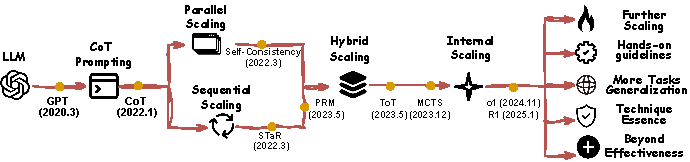
\includegraphics[width=.98\linewidth]{figures/figure1.pdf}
    \caption{From Emergence to the Next Frontier, the Evolutionary Path of Test-Time Scaling.}
    \label{fig:timeline}
\end{figure}





\begin{itemize}
    \item Crucially, these techniques are complementary rather than mutually exclusive: for instance, R1 necessitates an SFT-based warmup via rejection sampling. Therefore, achieving more powerful scaling requires systematically integrating these methods. Even within RL frameworks, practitioners should continue to leverage synthesized CoT approaches and incorporate structured inference strategies to tackle increasingly complex scenarios effectively.
    \item Researchers found that there does not exist one simple scaling solution that works for all problems. Increasingly, researchers tend to focus on optimal-scaling solutions~\citep{wu2024scaling,snell2024scaling}.
    \item The boundary between inference-based and tuning-based approaches is blurring. Consequentially, the target of scaling (\textit{what to scale}) changes between different stages. Certain papers, such as \citet{li2025draftsanswersunlockingllm, munkhbat2025selftrainingelicitsconcisereasoning}, tune the inference-based capability into the LLM by synthesizing high-quality data from inference-based approaches as the tuning data. Others, such as \citet{wan2024alphazero}, are proposing various techniques that better exploit the LLM's capability during both the training and inference stages.
\end{itemize}

